\documentclass[11pt,a4paper]{jsarticle}
%
\usepackage{amsmath,amssymb}
\usepackage{bm}
\usepackage{ascmac}
\usepackage[dvipdfmx]{graphicx}
%
\setlength{\textwidth}{\fullwidth}
\setlength{\textheight}{40\baselineskip}
\addtolength{\textheight}{\topskip}
\setlength{\voffset}{-0.2in}
\setlength{\topmargin}{0pt}
\setlength{\headheight}{0pt}
\setlength{\headsep}{0pt}
%
\newcommand{\writtenBy}[1]{\begin{flushright}文責: #1\end{flushright}~}
\newcommand{\divergence}{\mathrm{div}\,}  %ダイバージェンス
\newcommand{\grad}{\mathrm{grad}\,}  %グラディエント
\newcommand{\rot}{\mathrm{rot}\,}  %ローテーション
%
  \usepackage{listings,jlisting} 
  %ここからソースコードの表示に関する設定
  \lstset{
    basicstyle={\ttfamily},
    identifierstyle={\small},
    commentstyle={\smallitshape},
    keywordstyle={\small\bfseries},
    ndkeywordstyle={\small},
    stringstyle={\small\ttfamily},
    frame={tb},
    breaklines=true,
    columns=[l]{fullflexible},
    numbers=left,
    xrightmargin=0zw,
    xleftmargin=3zw,
    numberstyle={\scriptsize},
    stepnumber=1,
    numbersep=1zw,
    lineskip=-0.5ex
  }
  %ここまでソースコードの表示に関する設定

\title{競技プログラミング班 活動報告書}
\author{服部瑠斗 小村漱一朗 中野海人 稲垣和真 浜田直弥 西見元希 石川琉聖}
\date{\today}
\begin{document}
\maketitle
%
%
\section{活動の概要}
\writtenBy{稲垣 和真}
本プロジェクトは、競技プログラミングを通してプログラミングにおけるアルゴリ
ズムの知見を深めるために発足した。競技プログラミングに用いたツールはAtCoderであ
る。AtCoderのBeginner Contestや班内の活動内で開催したバーチャルコンテストを通し
て実際に問題を解き、その解法を活動で共有し、お互いの知見を高めたり、いろいろな
アルゴリズムの手法について会員が解説し、理解を深めるというものである。以上の2点
を主として本プロジェクトは活動した。

\section{競技プログラミングについて}
\writtenBy{稲垣和真}
競技プログラミングとは、解くべき問題が与えられ、その問題を解くプログラムを、早
く正確に解き、正解数や解くまでにかかった時間などを競う競技である。具体的には以
下の5つの要素からなる。
\begin{itemize}
    \item {\bf 問題文}
        \par
        解くべき問題の内容が記されている。
        \par
    \item {\bf 制約}
        \par
        問題文で出てきた数値や文字列に、どのような制約が与えられているかが記さ
        れている。
    \par
    \item {\bf 入力}
        \par
         入力は、標準入力にどのような形式で文字列を与えるかが記されている。
    \par
    \item {\bf 出力}
        \par
        標準出力にどのような形式で与えるかの条件が記されている。
    \par
    \item {\bf 入出力例}
        \par
        実際にプログラムに与えられる入力と、プログラムが出力すべき文字列が記されている。
\end{itemize}
\section{学習内容}

\subsection{アルゴリズム}
本プロジェクトでは以下の2つのアルゴリズムを学習した.
\begin{itemize}
    \item 深さ優先探索(dfs)
    \item 累積和
\end{itemize}

\subsubsection{深さ優先探索}
深さ優先探索とは、全探索を行うアルゴリズムの種類の一つである。
競技プログラミングでは主に、状態の遷移が分岐するような処理の実装に用いられている。
深さ優先探索の特徴として、与えられた状態の深さに注目して探索を行うという点が挙げられる。
また深さ優先探索を用いるメリットとして、再帰を用いて実装した場合コードがシンプルに記述することが出来るという点が挙げられる。

深さ優先探索の実装例

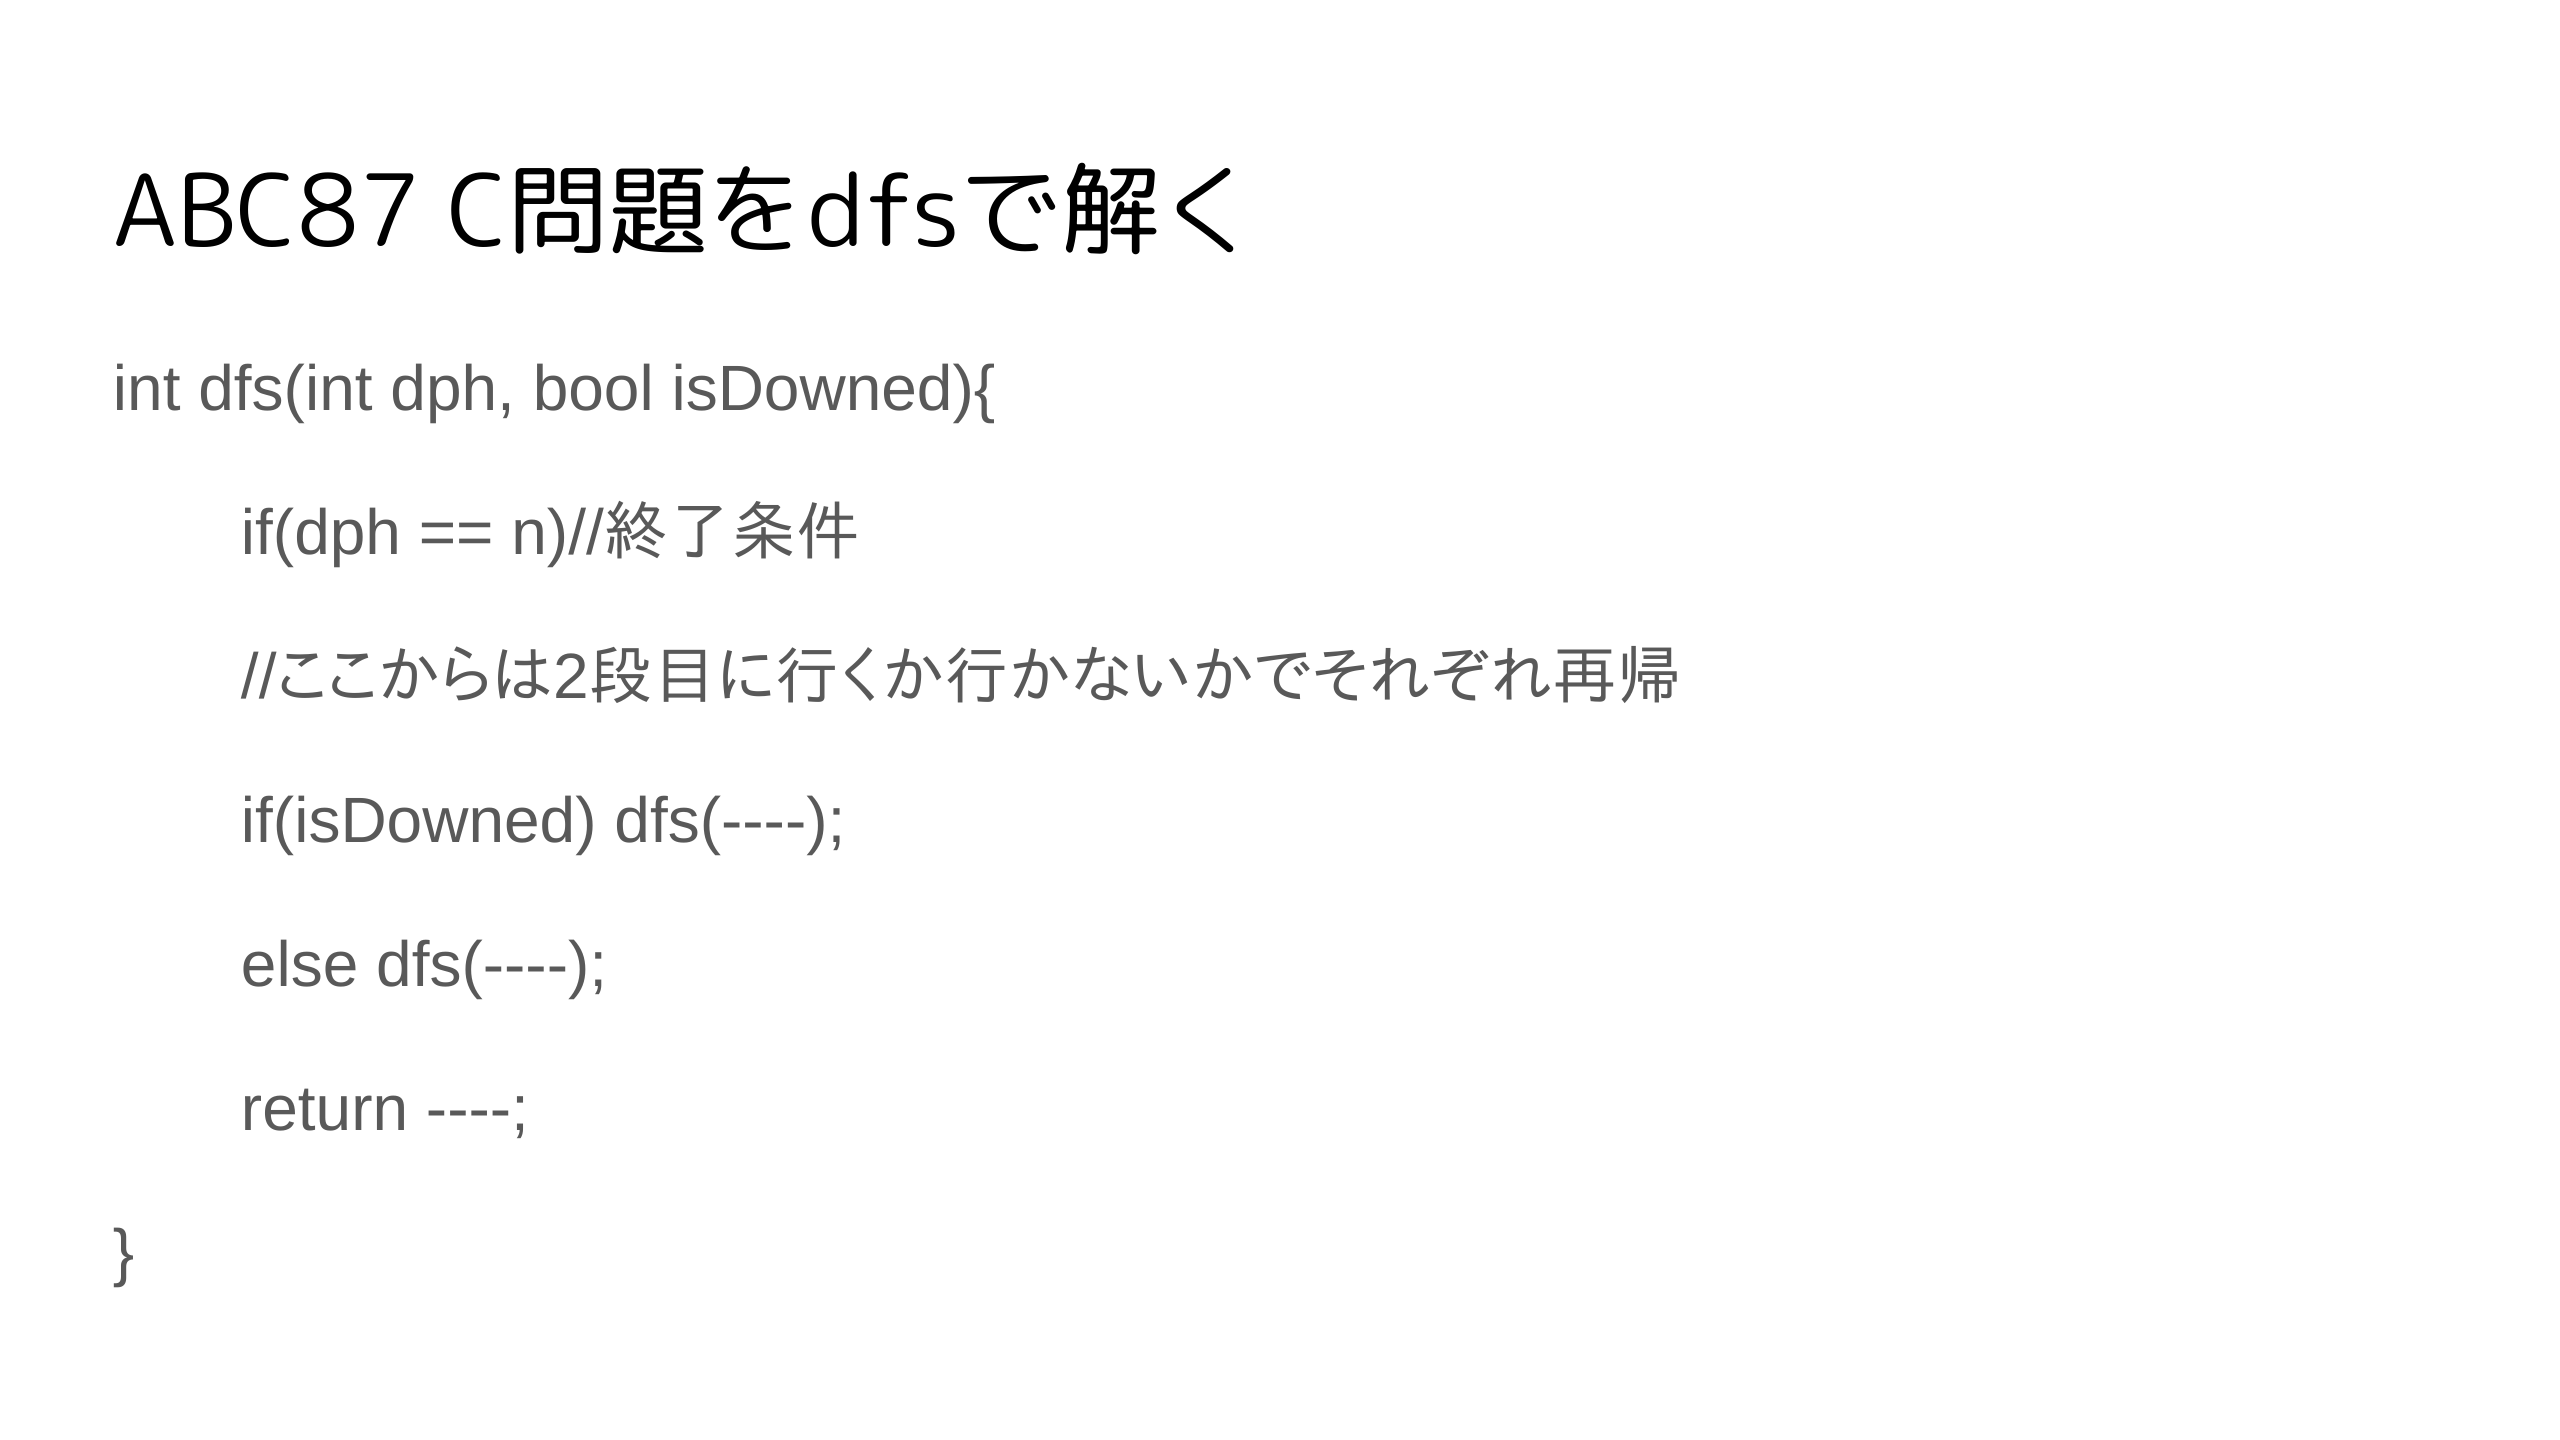
\includegraphics[width=10cm]{dfs.png}

\subsubsection{累積和}
累積和とは、計算量(オーダー)を圧縮するために用いられるアルゴリズムの種類の一つである。
競技プログラミングでは主に、配列上の区間の総和を求める処理の実装に用いられている。
累積和の特徴として、前処理を行うことによって元々の配列が保持している情報に加えてある区間の総和も求めることが出来るという点が挙げられる。

累積和の実装例.

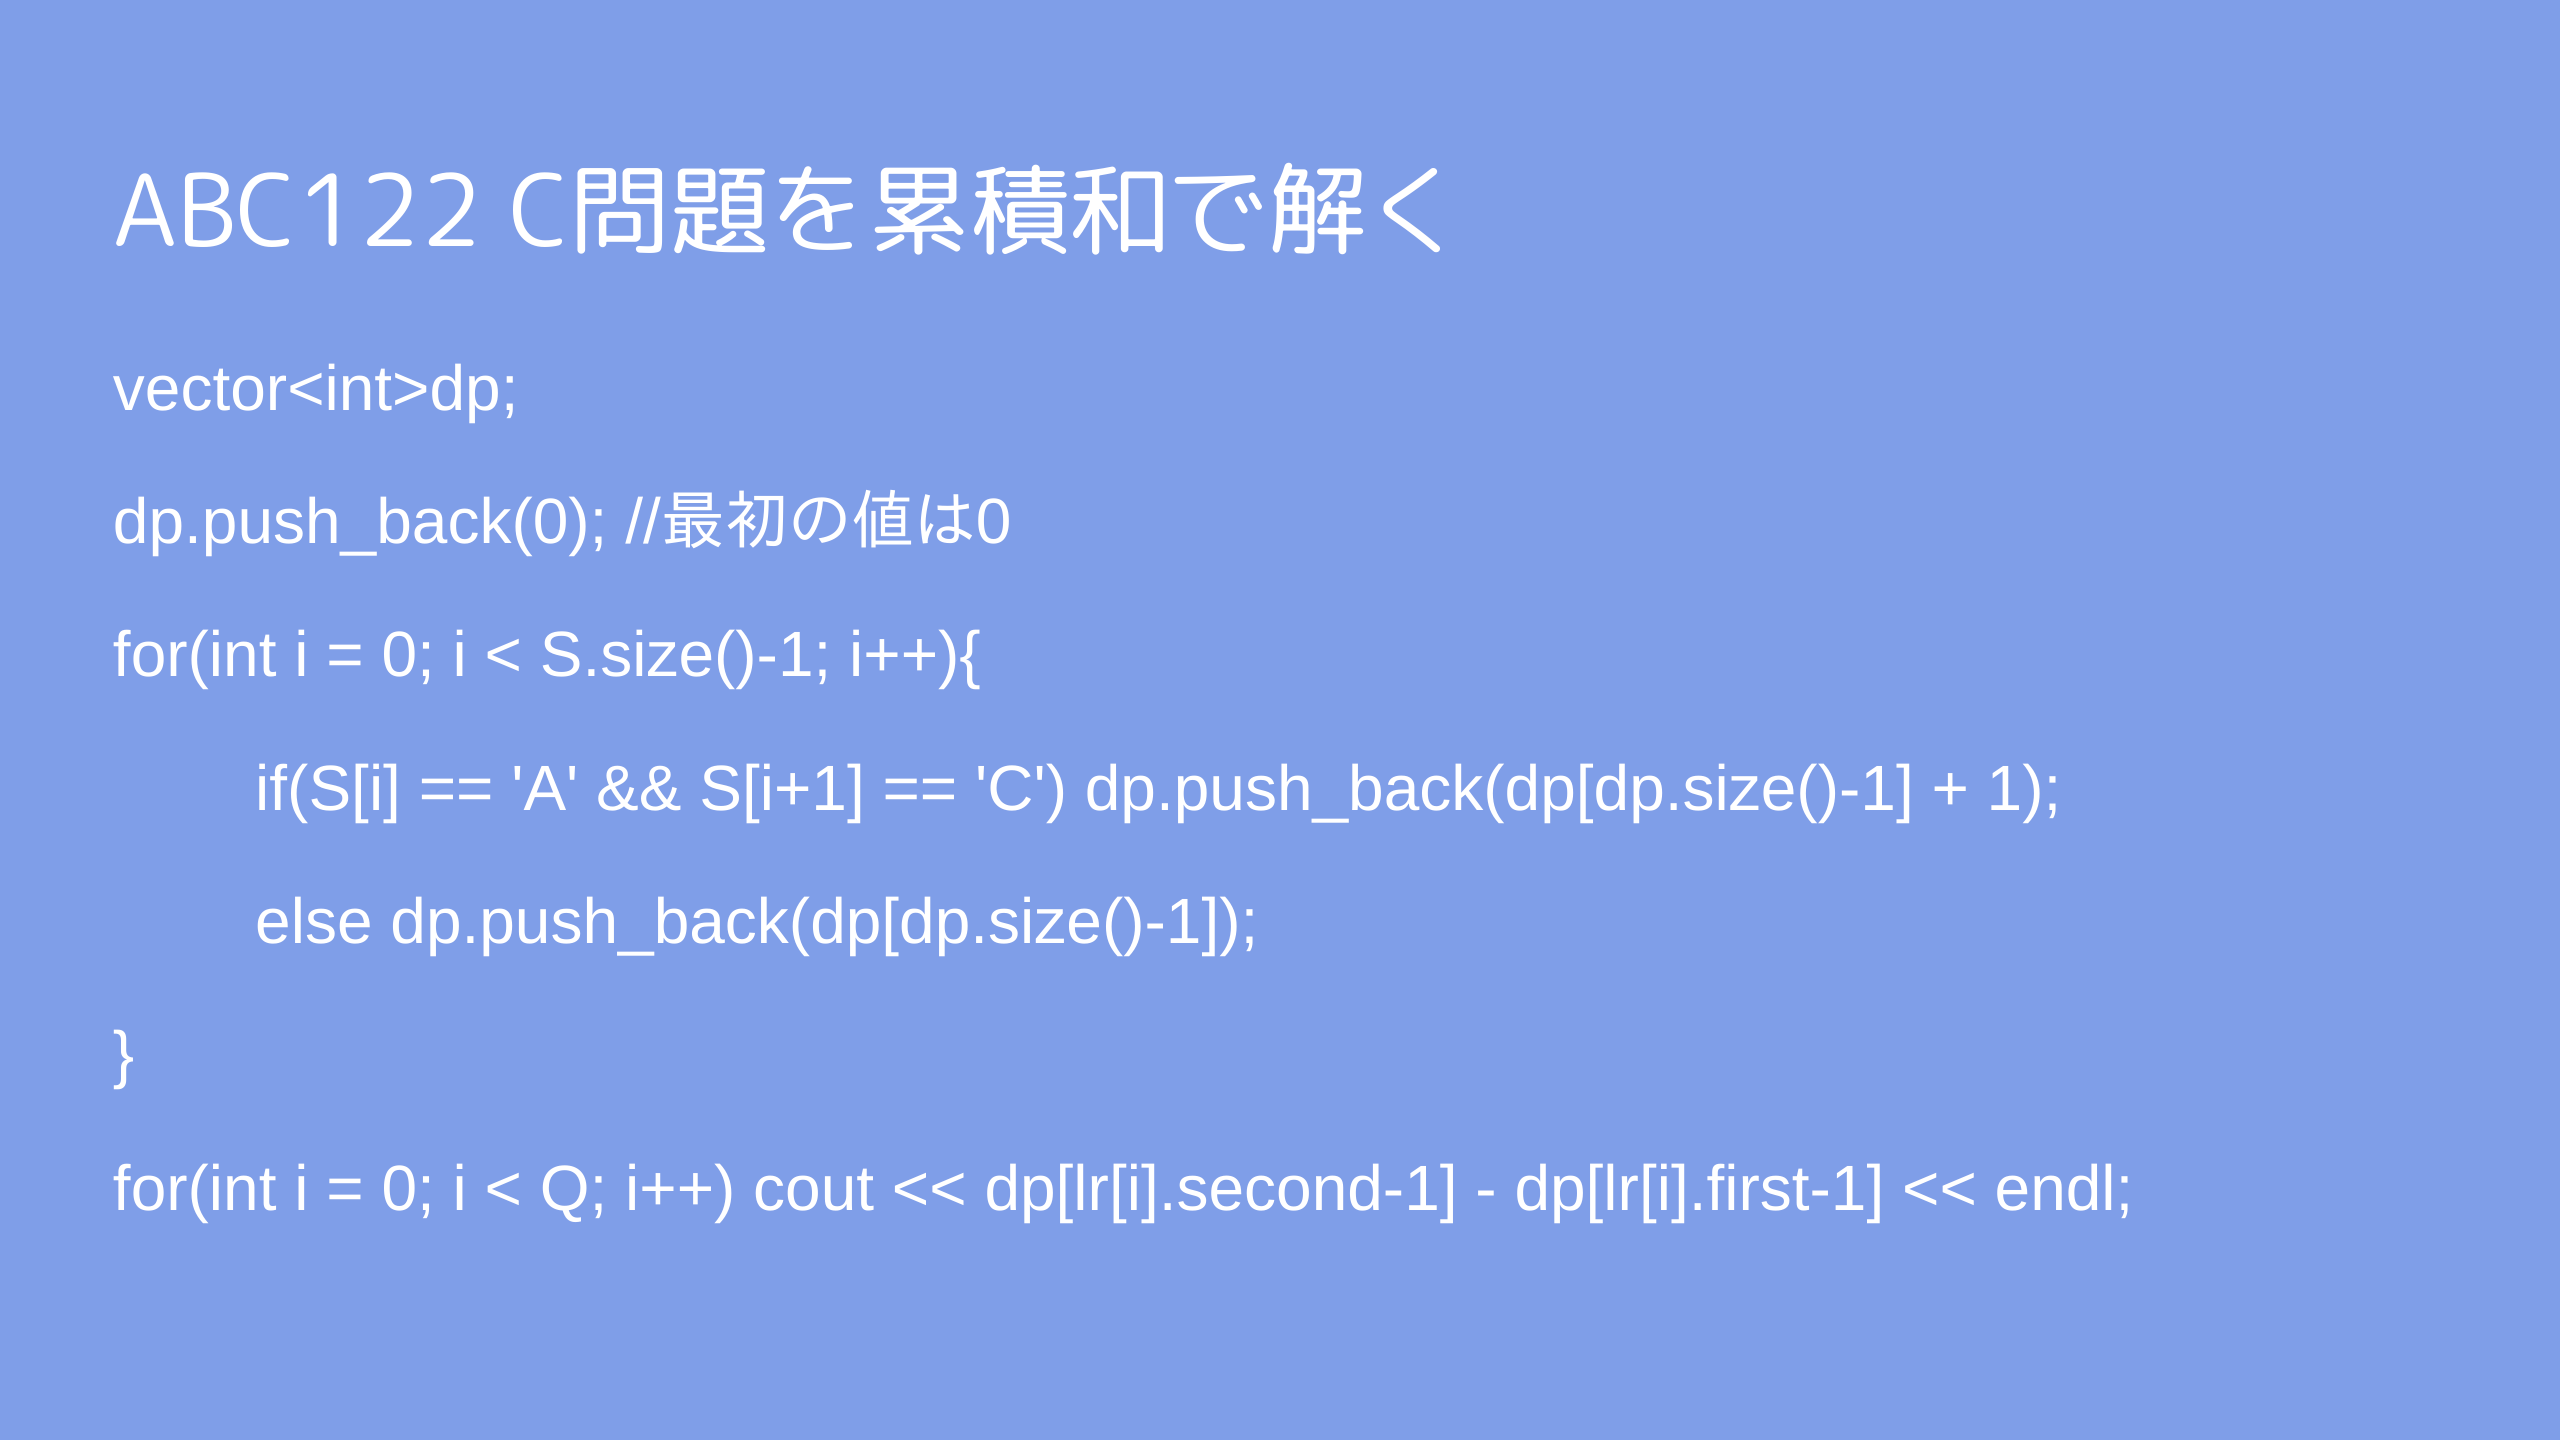
\includegraphics[width=10cm]{ruisekiwa.png}

\subsection{競技プログラミングにおけるテクニック}
\writtenBy{西見 元希}
%
本項では、この活動において学ぶことのできた競技プログラミングにおけるテクニックを述べる。
%
\begin{itemize}
    \item{\bf マクロの活用}
      \par
      defineマクロの活用は競技プログラミングにおける提出コードの冗長性を大きく削減し、より簡潔なコードを実現する。中でも単純な繰り返しにおけるrepマクロは最も頻繁に利用される。次のコードはrepマクロの定義と利用例、マクロを用いなかった場合との比較である。

  
%
  \begin{lstlisting}[caption=repマクロの例,label=fuga]
  #include<iostream>
  using namespace std;
 
  #define rep(i,n) for(int (i)=0;(i)<(n);++(i))
  
  //マクロを利用しない場合
  int main(void){
    int n=10;
    vector<int> a(n);
    for(int i=0;i<n;++i)
      a[i]=i;
    for(int i=0;i<n;++i)
      cout << a[i] << endl;
  }

  //マクロを利用した場合
  int main(void){
    int n=10;
    vector<int> a(n);
    rep(i,n) a[i]=10;
    rep(i,n) cout << a[i] << endl;
  }
  \end{lstlisting}
  このコードでは要素数10の可変長配列に要素の座標と同じ数値を格納しそれを出力しているが、repマクロを用いることでコードが短くなり可読性が向上したのが確認できるだろう。
      \par
    \item{\bf ラムダ式の活用}
      \par
      ラムダ式は関数型プログラミングにおいてよく用いられる言語機能であるが、競技プログラミングでの主流言語であるC++にもその機能があり、ソートなどの引数として極めて便利に利用することができる。次のコードはラムダ式を利用した整数列のソートの例である。
      \begin{lstlisting}[caption=lambda式の例]
      #include<bits/stdc++.h>
      using namespace std;
      int main(void){
        int n=10;
        vector<int> a(n);
        rep(i,n) a[i]=i;

        //降順にソート
        sort(v.begin(),v.end(),
          [](int x, int y) -> auto{return x>y;});

        //0246813579のようにソート
        sort(v.begin(),v.end(),
          [](int x, int y) ->
            auto {if(x%2==y%2)return x<y;
             else if(x%2)return x<y;
             else return x<y;});
      }
      \end{lstlisting}
      このようにラムダ式を用いたソートは非常に汎用的なソートが行える。
      \par
\section{活動で得られたもの}
本プロジェクトで得られたものは大きく2つに分けられる。

1つ目は、競技プログラミングの問題に対してどのアルゴリズムやテクニックを用いるかを判断する力である。
具体的には、制約を見ることによって判断することが出来る。理由としては制約から入力される値の上限が分かる。
上限の値が判明すればその値が入力された場合の最悪計算量(オーダー)を大まかに求めることが出来る。
最悪計算量が判明すれば、そこから全探索が出来るのか出来ないかといったアルゴリズムやテクニックの選択が可能になる。

2つ目は、アルゴリズムやテクニックを実際のコードに落としこみ問題を解く力である。
一般的にアルゴリズムやテクニックをただ学ぶだけでは実践で苦労してしまう。
そこで本プロジェクトでは、問題の内容を細分化することによって実践に落としこむ方法をいくつかプロジェクトメンバー間で共有することによって問題を解く力を習得した。

\section{問題点}
\section{展望}
\begin{thebibliography}
    \texttt{https://book.mynavi.jp/manatee/detail/id=56242}
\end{thebibliography}




%
%
\end{document}
